%\documentclass[11pt,a4paper]{book}
\documentclass[a4paper]{memoir}
%\documentclass{memoir}

\usepackage{titling}
\usepackage[utf8]{inputenc}
\usepackage[english]{babel}
\usepackage{mathtools}
\usepackage{hyperref}
\usepackage{booktabs}
\usepackage{graphicx}
\usepackage{caption}
\usepackage{subcaption}
\usepackage{xcolor}
\usepackage[]{rotating}
\usepackage[]{titlesec}
\usepackage[absolute]{textpos}




% Title Page
\title{SpiNNaker-based implementation of visual systems}
\author{Garibaldi~Pineda~García \\ Supervisor: Steve~Furber Co-supervisor: Dave~Lester}
\date{}

\definecolor{themecolor}{RGB}{80, 0, 127} %manchester
\definecolor{themecolordark}{RGB}{64, 26, 86} %dark-manchester
\definecolor{darkgray}{gray}{0.15}

\graphicspath{{./images/}}

\pagestyle{ruled}



\makechapterstyle{myBianchi}{%
  \chapterstyle{default}
  \setlength{\afterchapskip}{40pt}
  
  \renewcommand{\chapnamefont}{\normalfont\LARGE\itshape}
  \renewcommand{\chapnumfont}{\normalfont\LARGE}
  \renewcommand{\chaptitlefont}{\normalfont\Huge}

  \renewcommand{\printchaptername}{\chapnamefont\centering Chapter}

  \renewcommand{\printchapternum}{\chapnumfont \textit{\thechapter}}
  
  \renewcommand{\printchaptertitle}[1]{%
    \rule[5pt]{\textwidth}{0.4pt}\par
     \centering \chaptitlefont\textbf{##1} \\\mbox{}\rule[5pt]{\textwidth}{0.4pt}}


  \renewcommand{\printchapternonum}{%
    \vphantom{\chapnumfont \textit{9}}\afterchapternum}
  
  \renewcommand{\afterchaptertitle}{\par\nobreak\vskip \afterchapskip}

}

\chapterstyle{myBianchi}



\begin{document}

  \pagenumbering{gobble}
  \thispagestyle{empty}
  \setlength{\TPHorizModule}{1mm}
\setlength{\TPVertModule}{1mm}
%\begin{titlepage}
  ~
  \begin{textblock}{50}(175,0)
    \begin{color}{themecolor}
      \rule{3cm}{30cm}
    \end{color}
  \end{textblock}

  \begin{textblock}{160}(-10,33)
    \begin{color}{themecolor}
      \rule{18.4cm}{2.2cm}
    \end{color}
  \end{textblock}
  
  % Logo white
  \begin{textblock}{150}(20,30)
    \begin{flushright}
    %\rule{2cm}{2cm}\\[2em]   
    \includegraphics[height=20mm]{manchester-logo}\\[5em]
    
    {\noindent\Huge\bfseries SpiNNaker-based Visual Systems}\\[2em]
    
    {\noindent\huge End-of-first-year report }\\[5em]
    
    {\noindent\Large\bfseries Garibaldi~Pineda~García}\\[0.5em]
    {\noindent\Large Supervisor: Steve~Furber}\\[0.1em]
    {\noindent\Large Co-supervisor: Dave~Lester}\\[1em]
    {\noindent\large Advanced Processing Technologies Group\\
      School of Computer Science \\
      University of Manchester\\[0.4em]
      United Kingdom}
    \end{flushright}
  \end{textblock}
  
  
  \begin{textblock}{20}(186,285)
    \begin{rotate}{90}
      %{\huge\sffamily\bfseries \textcolor{white}{University of Manchester}}
      {\huge\bfseries \textcolor{white}{University of Manchester}}
    \end{rotate}
  \end{textblock}
  \begin{textblock}{20}(196,285)
    \begin{rotate}{90}
      %{\huge\sffamily\bfseries \textcolor{white}{University of Manchester}}
      {\huge\bfseries \textcolor{white}{APT Group}}
    \end{rotate}
  \end{textblock}  

  \begin{textblock}{150}(20, 250)
    \begin{flushright}
    \includegraphics[height=30mm]{spinnaker-logo}
    \end{flushright}
  \end{textblock}
  
%\end{titlepage}



  \cleardoublepage
  \pagenumbering{gobble}
  \tableofcontents
  \cleardoublepage
  \pagenumbering{arabic}


  \chapter{Introduction}
  \section{Neural codes and vision}
\section{Common cameras as spike train sources}
  \label{chp:intro}

  \chapter{A look into the brain}
  \label{chp:brain}
  \section{Introduction}
\section{Neurons and responses}
\section{Coding schemes}
\section{Conclusions}

  \chapter{Vision}
  \label{chp:vision}
  Vision is one of the most important senses for animals; humans use it extensively for all kinds of tasks. Hunting, assessing danger, reading, driving, drawing, predicting rain from grey clouds, etc., these are all tasks that involve \emph{seeing}. There is a vast collection of knowledge about the components of vision (primates in particular), though a unification (or the answer to \emph{How do we see?}) has not yet been achieved.

Artificial neural networks have been used to emulate some behaviours of the human visual system. One of the most successful is image recognition, in particular using deep networks~\cite{deep-nets-hinton2006fast,krizhevsky2012imagenet}. Seminal computer vision research has also been based on the functional characteristics of biological vision~\cite{lowe1999object,lowe2004distinctive,alahi2012freak}. The success of bio-inspired research in computer vision is the inspiration for studying the visual pathway in animals (primates in particular) and to create a system that would solve the SLAM problem.

\section{The eye and the retina}
\label{sec:vision:eye}
Our everyday experience might lead us to believe that the eyes are sensory organs developed completely separate from the brain but, in fact, the retina is an extension of the brain that performs spatio-temporal compression of a continuous flow of ``images'' of the world~\cite{eye-brain-vision-hubel1995}.

The eye is composed of many parts that resemble a mechanical camera (Figure~\ref{fig:vision:eye}). The cornea is a transparent film that protects the frontal part of the eye and encloses the eye. The lens is in charge of focusing light rays into the retina, which acts as a complex sensor that will be described further in the following paragraphs. The pupil and the iris act as a camera's aperture mechanism, the amount of light input is regulated by broadening or reducing the diameter of the pupil. 

\begin{figure}[htb]
  \begin{center}
    \includegraphics[width=0.5\textwidth]{simple-eye-anatomy}
    \caption{Simplified anatomy of the eye~\cite{webvision-images}.}
    \label{fig:vision:eye}
  \end{center}
\end{figure}

The retina is organized in layers of cell bodies or nerves,  Figure~\ref{fig:vision:simple-retina} shows a simplified version of the retina's anatomy~\cite{webvision-simple-retina}. Light enters the eye and has to travel all the way to the deepest part of the retina (right of Fig.~\ref{fig:vision:simple-retina}) to be sensed by the photoreceptors. 

\begin{figure}[h]
  \begin{center}
    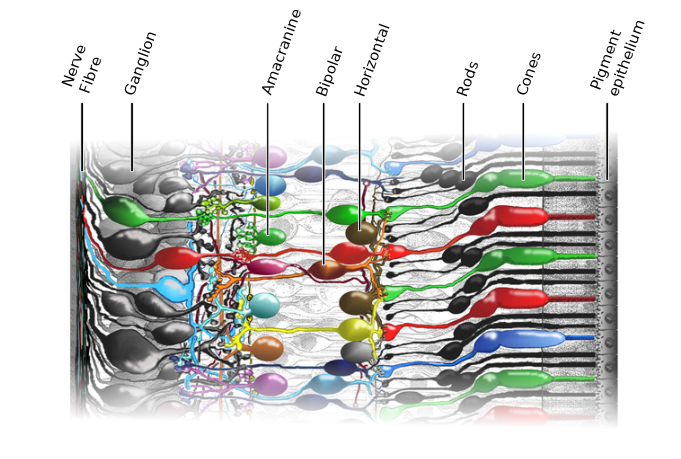
\includegraphics[width=0.7\textwidth]{retina-simple}
    \caption{Simple anatomy of the retina, adapted from~\cite{webvision-images}.}
    \label{fig:vision:simple-retina}
  \end{center}
\end{figure}

Photoreceptors transform light into an electrical signal. There are two primary types of photoreceptor cells within the retina: Colour is perceived by special type of receptors \emph{cones} and, contrast is perceived by \emph{rods}. Many mammals have retinas with more rods than cones, but primates' retinas are split in two separate zones. Most of the photosensitive area has more rods than cones but in a tiny region called the \emph{foveal pit}, there are almost no rods -- it's densely packed with cones. It is used for high-resolution vision and is virtually useless when there is not enough light~\cite{eye-brain-vision-hubel1995}.

The precise function of the other cell types is still a matter of debate and research. What is known is that \textbf{horizontal} cells  spatially average the input from photoreceptors and transmit to bipolar, which in turn output to ganglion cells. Horizontal cells also send a feedback signal to the photoreceptors, perhaps to adapt to different light conditions. \textbf{Bipolar} cells, as their name suggests, have outputs both to ganglion cells and photoreceptors. These first cell types (photoreceptors, horizontal and bipolar cells) use analog signals and feed ganglion cells which have a \emph{centre-surround} behaviour~\cite{eye-brain-vision-hubel1995,thompson2000brain}. Figure~\ref{fig:vision:centre-surround} illustrates the reaction of the two variants of centre-surround cells to different inputs.

\begin{figure}[h]
  \begin{center}
    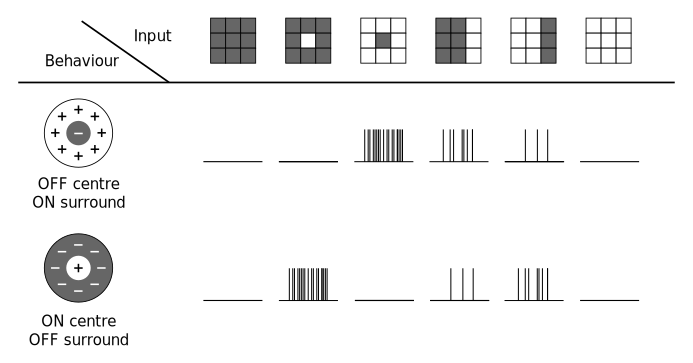
\includegraphics[width=0.7\textwidth]{centre-surround}
    \caption{Responses of centre-surround cells to different types of input.}
    \label{fig:vision:centre-surround}
  \end{center}
\end{figure}


\textbf{Ganglion} cells take input from bipolar cells, some form the surround (signal adapted by horizontal cells) and others the centre (pure signal from the photoreceptors). The centre-surround behaviour has been modelled by many authors using \emph{Laplacian of Gaussians} or \emph{Difference of Gaussians} ~\cite{thorpe-rate-coding-theory,virtual-retina,webvision-midget}. The output of ganglion cells are action potentials which are transmitted by the ganglion's axons, into the Lateral Geniculate Nucleus (LGN).

It's likely that most of the information sensed by the retina is redundant, this would keep the eyes working adequately even if some cells cease to function. To avoid saturation of nerve fibres and over-representation, lateral inhibition might play a big role~\cite{basab-model,thorpe-rate-coding-theory,field-sensory-coding}. The use of centre-surround responses in the retina is believed to help the eye overcome variations in lightning conditions, because the response comes from the contrast comparison between photoreceptors.

%After the light rays have been encoded into a neural representation, the optic nerve transfers the information to the Lateral Geniculate Nucleus (LGN) and from there to the visual portion of the cortex. A huge difference between a camera and the eye is that the latter maintains a continuous stream of information unlike the frame-based nature of cameras.

\section{The visual cortex}
\label{sec:vision:cortex}
At the end of last section, we stated that information from ganglion cells extend to the Lateral Geniculate Nucleus (LGN), where information is relayed and organized so that the cortex can interpret it. Organization makes left visual field sent to right hemisphere, right field to left hemisphere (Figure~\ref{fig:vision:optic-chiasm}).

\begin{figure}
  \begin{center}
    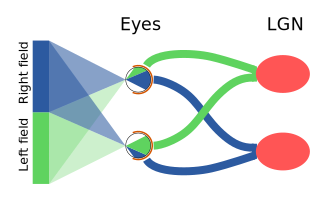
\includegraphics[width=0.7\textwidth]{visual-fields-lgn}
    \caption{Visual field mapping in LGN.}
    \label{fig:vision:optic-chiasm}
  \end{center}
\end{figure}

The portion of the cortex that is involved with visual processing has been estimated to about 30\%.

It has been studied and areas have been labelled due to their function.

V1, 
The primary visual cortex (V1) is the best-studied visual area in the brain.
correspondence between a given location in V1 and in the subjective visual field is very precise
 fovea in the retina, a large portion of V1 is mapped to the small, central portion of visual field
neuronal responses can discriminate small changes in visual orientations, spatial frequencies and colors. 
described as edge detection. 

V2
connections from v1 sends to v3,v4,v5 back to b1
more complex shapes than v1

V3
controversy still exists regarding the exact extent of area V3,
 it may contain a complete visual representation
  may play a role in the processing of global motion
  
V4
strong feedforward input from V2 and sending strong connections to the PIT
receives direct inputs from V1, especially for central space
it has weaker connections to V5 and dorsal prelunate gyrus (DP).
show strong attentional modulation
orientation, spatial frequency, and color.
tuned for object features of intermediate complexity, like simple geometric shapes
V4 is not tuned for complex objects such as faces, as areas in the inferotemporal cortex are

V5
Visual area V5, also known as visual area MT (middle temporal), is a region of extrastriate visual cortex that is thought to play a major role in the perception of motion, the integration of local motion signals into global percepts, and the guidance of some eye movements.


V6
sharp selectivity for the orientation of visual contours, and preference for long, uninterrupted lines covering large parts of the visual field
strongly responsive to low spatial frequency components of an image, and respond poorly to the motion of textured pattern


\section{Artificial neural networks}
inspired by biological nervous sys
graph model
nodes interconnected "neurons" which send messages to each other
learn statistics about input
edges contains sets of adaptive weights modified by learning algo

function approximation, classification, robotics, pattern recognition

Artificial neural networks (ANN) first appeared as a novel way of solving problems that was inspired by the way the brain computes~\cite{mcculloch1943logical}. Generations of neural networks can be classified by their basic compute unit, the neuron model. Under this scheme, the \textbf{first generation} used \textsc{on-off} threshold gates, also known as perceptrons. The basic functionality is that if the input value is above a certain threshold, the neuron will output a 1 and 0 otherwise. These type of network is limited to binary outputs. First generation ANN are able to compute every boolean function using a single hidden layer~\cite{third-gen-nn-Maass1997}.

The \textbf{second generation} of neural models make use of an activation function which enables the output of analog values. The typical activation function is a sigmoid (eq. \ref{eq:neuro:sigmoid}). Whenever the activation function reaches a certain threshold, the neuron will be ``fire''.

\begin{equation}
  \sigma(x) = \frac{1}{1 + e^{-x}}
  \label{eq:neuro:sigmoid}
\end{equation}

A notable addition is that multi-layered network of the second generation are able to be trained using gradient descent-based algorithms~\cite{hecht1989-backprop-theory}. One drawback is that they are not biologically plausible, for they can be interpreted as neurons using rate coding which is an unlikely candidate for fast computations in the brain~\cite{third-gen-nn-Maass1997}.

Spiking neural networks are considered the \textbf{third generation} of ANN, the main difference is that their activation function is closer to the one observed in biological neurons. Some neuron models used were described in previous sections. Third generation ANN are able to approximate any analog continuous function~\cite{third-gen-nn-Maass1997}. 
%\begin{figure}
%  \begin{center}
%    \begin{subfigure}{0.25\textwidth}
%      %    \vspace*{0.8em}
%      \centering
%      \captionsetup{justification=centering}
%      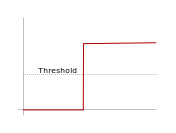
\includegraphics[width=\textwidth]{perceptron}
%      \caption{Perceptron}
%      \label{fig:neuro:perceptron}
%    \end{subfigure}
%    \begin{subfigure}{0.25\textwidth}
%      %    \vspace*{0.8em}
%      \centering
%      \captionsetup{justification=centering}
%      \includegraphics[width=\textwidth]{sigmoid}
%      \caption{Sigmoid}
%      \label{fig:neuro:sigmoid}
%    \end{subfigure}
%    \begin{subfigure}{0.265\textwidth}
%      \centering
%      \captionsetup{justification=centering}
%      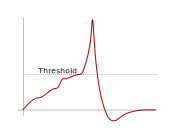
\includegraphics[width=\textwidth]{spike}
%      \caption{Spike}
%      \label{fig:neuro:spike-func}
%    \end{subfigure}
%  \end{center}
%\end{figure}
There are some synaptic learning rules for spiking neural networks, the most studied one being Spike-Timing-Dependant Plasticity (STDP)~\cite{STDP-Song2000}. 
It follows a Hebbian philosophy, \emph{neurons that fire together, wire together}~\cite{hebb2005organization}. The basic idea is that when a post-synaptic spike is generated nearly after a pre-synaptic one, the connection is between this pre and post neurons is strengthened.\\

If the network topology is also taken into the classification basis, a new generation can be added. \emph{Deep networks} are thought to be the \textbf{fourth generation} of neural networks. Previously, researchers had tried to train deep networks but found that it was a difficult task to achieve for more than one hidden and it actually decreased the performance of the network~\cite{learning-deep-Bengio2009}. In 2006, \citeauthor{hinton2006fast} report an algorithm to train deep architectures without supervision, one layer at a time; the authors named their network a \emph{Deep Belief Network} (DBN). After this seminal work, other researchers used the same one layer at a time  approach but with different learning algorithms. While \citeauthor{hinton2006fast} used restricted Boltman machines (RBM), \citeauthor{autoencoders-lecun2007} used auto-encoders~\cite{autoencoders-lecun2007}. Since these learning techniques use real numbers as values and not \textsc{on-off} responses as spiking neural networks, the use of deep architectures in the latter has been limited. The usual path is to train a network off-line, transfer the weights to an equivalent SNN and use that as the energy-efficient on-line application~\cite{evangelos-deep-belief,diehlfast-deep-net}.

\section{Visual cortex models}
Lowe's work inspired by neuro

Hierarchical has been shown to provide geometric transformation invariance

Hierarchical neural networks for image interpretation

Hierarchical temporal memory 

\section{Conclusions}
\label{sec:vision:conclusions}
\section{Conclusion}
\section{Further work}
\section{Plans for second and third year}


  \chapter{Neuromorphic hardware}
  \label{chp:neuro-hw}
  \section{Introduction}
\section{Classic computing}
\section{Neuromorphic trends}
\section{Event-based model}
\section{SpiNNaker}
\section{Conclusions}

  \chapter{From images to spikes}
  \label{chp:img2spk}
  \section{Real-time encoding}
For mobile and robotics applications a real-time encoder is needed. Hardware based real-time video encoders are expensive and not massively produced, thus their availability is limited. Creating one with off-the-shelf components opens the potential users. Two different models chosen whose computational cost was low enough to keep them operating at real-time and had kept biological plausibility constraints.


\subsection{General purpose computing in the graphics processor unit}

GPU History
GPU programming 
OpenCL
Memory hierarchy

\subsection{The foveal pit model}

The highest resolution area of the eye is the foveal pit (see section \ref{sec:vision:eye}). A functional model for this region of the retina was developed by \citeauthor{basab-model}, they called the implementation the \emph{Filter-overlap Correction algorithm} (FoCal)\cite{basab-model}. It's based on the response and physiology of the fovea. The authors concluded that using four different layers of ganglion cells, most of the visually relevant information could be recovered after encoding. Furthermore, the encoder outputs a collection of rank-ordered spike trains. 

The ganglion cells themselves where modelled using Difference of Gaussians (DoG), Equation \ref{eq-dog}. 

\begin{equation}
\label{eq-dog}
DoG_w(x,y) = \pm\frac{1}{2\pi\sigma_{w,c}^2}e^{\frac{-(x^2 + y^2)}{2\sigma_{w,c}^2}}
\mp\frac{1}{2\pi\sigma_{w,s}^2}e^{\frac{-(x^2 + y^2)}{2\sigma_{w,s}^2}}
\end{equation}

The size of the receptive field of the simulated cells depends on the layer they belong to, this is reflected in the convolution kernel's width and parameters. Variables $\sigma_{w,c}$ and $\sigma_{w,s}$ are the standard deviation for the centre and surround components of the DoGs for layer $w$.  The signs for the equation will be ($-$,$+$) if the ganglion cell is \emph{off-centre} and ($+$,$-$) if it is \emph{on-centre}. The parameters for this equation can be found in table \ref{tab-kernel-specs}.

\begin{table}[htb]
  \caption{Simulation parameters for ganglion cells}
  \centering
  \bgroup
  \def\arraystretch{1.4}
  
  %  \begin{TAB}(r,1em,1.5em){|c|c|c|c|c|}{|c|c|c|c|c|} 
  \begin{tabular}{c c c c c c}
    \begin{minipage}{1cm}Layer \end{minipage}& 
    \begin{minipage}{2cm}Behaviour \end{minipage}&
    \begin{minipage}{1cm} \centering Matrix width \end{minipage}&  
    \begin{minipage}{2.5cm}\centering Centre \\std. dev. ($\sigma_c$)\end{minipage} & 
    \begin{minipage}{2.5cm}\centering Surround \\std. dev. ($\sigma_s$)\end{minipage} & 
    \begin{minipage}{2.5cm}\centering Sampling resolution \\(cols, rows)\end{minipage} \\
    \hline
    \begin{minipage}{1cm}\vspace*{0.1cm} \centering1 \end{minipage} &
    \begin{minipage}{2cm}\textsc{off}-centre \vspace*{0.005cm} \end{minipage}& 
    \begin{minipage}{0.5cm}\centering$3$ \end{minipage}& 
    $0.8$ & $6.7 \times \sigma_c$ & 1, 1\\
    \begin{minipage}{1cm}\centering 2 \end{minipage} & 
    \begin{minipage}{2cm}\textsc{on}-centre \vspace*{0.005cm}\end{minipage} & 
    \begin{minipage}{0.5cm}\centering $11$ \end{minipage}& 
    $1.04$ & $6.7 \times \sigma_c$ &  1, 1\\
    \begin{minipage}{1cm}\centering 3 \end{minipage} &
    \begin{minipage}{2cm}\textsc{off}-centre \vspace*{0.005cm}\end{minipage} & 
    \begin{minipage}{1cm}\centering $61$ \end{minipage}& 
    $8$ & $4.8 \times \sigma_c$ & 5, 3 \\
    \begin{minipage}{1cm}\centering 4 \end{minipage} & 
    \begin{minipage}{2cm}\textsc{on}-centre \vspace*{0.005cm}\end{minipage} & 
    \begin{minipage}{0.5cm}\centering $243$\end{minipage} &
    $10.4$ & $4.8 \times \sigma_c$ & 5, 3
  \end{tabular}
  \label{tab-kernel-specs}
  \egroup
  \vspace*{-5pt}
\end{table}

For each cell type, a convolution kernel must be computed and stored in a matrix ($DoG_{w}$). For each element in the matrix we use Equation \ref{eq-dog}, substituting parameters specified in Table \ref{tab-kernel-specs} and integer valued $x$-$y$ coordinates whose origin is the centre of the matrix. For example, for the $3\times3$ kernel (layer 1 cells), the upper-left value would be calculated as follows:

\begin{align}
\label{eq-dog-3x3}
DoG_3(x,y) &= -\frac{1}{2\pi\sigma_{3,c}^2}e^{\frac{-(x^2 + y^2)}{2\sigma_{3,c}^2}}
+ \frac{1}{2\pi\sigma_{3,s}^2}e^{\frac{-(x^2 + y^2)}{2\sigma_{3,s}^2}} \\
DoG_3(-1,-1) &= -\frac{1}{2\cdot\pi\cdot 0.8^2}e^{\frac{-((-1)^2 + (-1)^2)}{2\cdot 0.8^2}}
+ \frac{1}{2\cdot\pi\cdot 5.36^2}e^{\frac{-((-1)^2 + (-1)^2)}{2\cdot 5.36^2}} \nonumber \\[0.5em]
             &= 0.27399398 \nonumber
\end{align}

The procedure to encode images can be broken into two parts. First, algorithm \ref{code-focal-conv} simulates the ganglion cells. It requires four independent 2D convolutions (Eq. \ref{eq-convolution}) using DoG kernels calculated as explained in the previous paragraph. 

\begin{equation}
\label{eq-convolution}
C(x,y,w) = I \ast DoG_w = \sum_i \sum_j \left( I(i+x, j+y) \cdot DoG_w(i,j)\right)
\end{equation}

\begin{algorithm}[h]
  \caption{FoCal, Part 1}
  \label{code-focal-conv}
  \begin{algorithmic}
    \Procedure{GanglionCells}{image $I$, kernels $DoG$}
    \State $C \leftarrow \emptyset$
    \ForAll{$w \in Layers$}
    \State $C \leftarrow C \cup I \ast DoG_w$
    \EndFor
    \State \textbf{return} $C$
    \EndProcedure
    \algstore{bkbreak}
  \end{algorithmic}
\end{algorithm}

We'll call coefficients to the pixel values that come out of the convolutions (Figures \ref{pic-lena-M-OFF}, \ref{pic-lena-M-ON}, \ref{pic-lena-P-OFF} and \ref{pic-lena-P-ON}). This coefficients are interpreted as a quantity that is inversely proportional to the spike emission time. That is, the pixel with the largest coefficient value represents the ganglion cell that will spike first.

\begin{figure}[hbt]
  \centering
  \begin{subfigure}[t]{0.32\textwidth}
    \centering
    \captionsetup{justification=centering,margin=0.1cm}
    \includegraphics[width=\textwidth]{./Lena-gray}
    \caption{Original image}
    \label{pic-lena}
  \end{subfigure}
  \begin{subfigure}[t]{0.32\textwidth}
    \centering
    \captionsetup{justification=centering,margin=0.1cm}
    \includegraphics[width=\textwidth]{./Lena-midget_off}
    \caption{Layer 1}
    \label{pic-lena-M-OFF}
  \end{subfigure}
  \begin{subfigure}[t]{0.32\textwidth}
    \centering
    \captionsetup{justification=centering,margin=0.1cm}
    \includegraphics[width=\textwidth]{./Lena-midget_on}
    \caption{Layer 2}
    \label{pic-lena-M-ON}
  \end{subfigure}
  \begin{subfigure}[t]{0.32\textwidth}
    \vspace*{0.8em}
    \centering
    \captionsetup{justification=centering,margin=0.1cm}
    \includegraphics[width=\textwidth]{./Lena-parasol_off}
    \caption{Layer 3}
    \label{pic-lena-P-OFF}
  \end{subfigure}
  \begin{subfigure}[t]{0.32\textwidth}
    \vspace*{0.8em}
    \centering
    \captionsetup{justification=centering,margin=0.1cm}
    \includegraphics[width=\textwidth]{./Lena-parasol_on}
    \caption{Layer 4}
    \label{pic-lena-P-ON}
  \end{subfigure}
  \caption{Results of simulating ganglion cell layers (convolved images were enhanced for better contrast)}
  \label{fig-convolution-results}
\end{figure}

In order to check the validity of the generated spikes, a reconstruction procedure is employed (Equation \ref{eq:reconstruction}). Each coefficient in $C$ has an origin layer $w$, a value $c$ and a position ($k$, $l$). For all coefficients in $C$, a DoG from it's respective layer will be weighed by it's value and be added at the it's position to the reconstructed image $R$. The procedure is based on the assumption that the DoG are orthogonal basis. Figure \ref{pic-unfiltered-spikes} shows the result of the image reconstruction procedure without any redundancy correction applied.

\begin{equation}
  R(x,y) = \sum_{i}^{} \sum_{j}^{} \sum_{w}^{} C_{w}(i - x, j - y)DoG_{w}(i, j)
  \label{eq:reconstruction}
\end{equation}

\begin{figure}[hbt]
  \centering
  \begin{subfigure}[t]{0.3\textwidth}
    \centering
    \captionsetup{justification=centering,margin=0.1cm}
    \includegraphics[width=\textwidth]{./Lena-gray}
    \caption{Original image}
  \end{subfigure}
  \begin{subfigure}[t]{0.3\textwidth}
    \centering
    \captionsetup{justification=centering,margin=0.1cm}
    \includegraphics[width=\textwidth]{./final_results-unfiltered}
    \caption{100\% of raw spikes}
    \label{pic-unfiltered-spikes}
  \end{subfigure}
  \caption{Reconstruction results without overlap correction.}
\end{figure}

The eye is unlikely to provide unnecessary information to the brain, that is redundant information is filtered somehow before it's delivered. In the retina, lateral inhibition is the most likely candidate to minimize information redundancy. It's still a matter of discussion where and by which cells is lateral inhibition performed in the retina. It is most likely to happen in layers prior to the ganglion cell layer. The DoG kernels are only an approximately orthogonal basis, thus the resulting coefficients from the convolutions in Algorithm \ref{code-focal-conv} suffer from redundant information. That is, two neighbouring pixels might contain information that represent the same feature in the image. The main issue with this redundancy is that neighbouring coefficients might encode almost the same information with a similar value. Since the value provides the order of the spikes, this phenomenon will push other important coefficients into the later, less important, parts of the spike representation. In order to correct for redundancy, FoCal performs a second step (Algorithm \ref{code-focal-corr}).

\begin{algorithm}[htb]
  \caption{FoCal, Part 2}
  \label{code-focal-corr}
  \begin{algorithmic}
    \algrestore{bkbreak}
    \Procedure{Correction}{coeffs $C$, correlations $Q$}
    \State $N \leftarrow \emptyset$ \Comment{Corrected coefficients}
    \Repeat
    \State $m \leftarrow max(C)$
    \State $M \leftarrow M \cup m$
    \State $C \leftarrow C \setminus m$
    \ForAll{$ c \in C$} \Comment{Adjust all remaining c}
    \If{$Q(m, c) \neq 0$} \Comment{Adjust only near}
    \State $c \leftarrow c - m \times Q(m, c)$
    \EndIf
    \EndFor
    \Until{$C = \emptyset$}
    \State \textbf{return} $M$
    \EndProcedure
  \end{algorithmic}
\end{algorithm}

All the coefficients that where obtained from Algorithm \ref{code-focal-conv}, are put in a set $C$. For every step of the correction procedure the maximum coefficient is searched and its spatially surrounding pixels in all layers (Figure \ref{fig:focal2}) will be adjusted according to the correlation due to overlap between the maximum coefficient's convolution kernel and the other layer's kernels. The bold square in Figure \ref{fig:overlap} shows the overlap of two $3\times3$ kernels of neighbouring pixels, a similar overlap is considered for the interaction between layers.
\begin{figure}[htb]
  \centering
  \begin{subfigure}[t]{0.68\textwidth}
  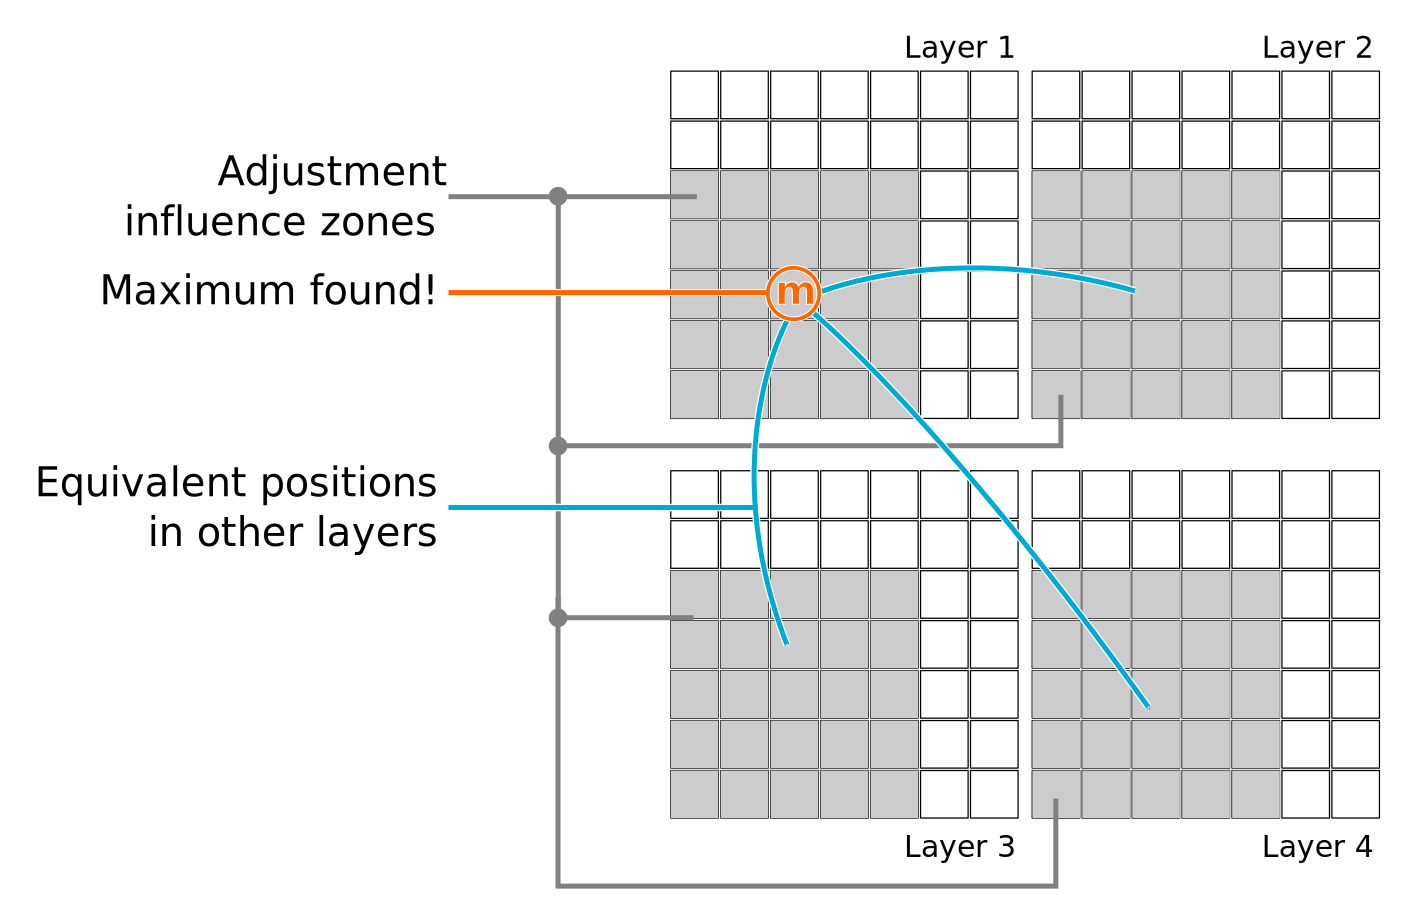
\includegraphics[width=\textwidth]{correction_adjustment}
  \caption{FoCal correction influence zones.}
  \label{fig:focal2}
  \end{subfigure}
  \hfill
  \begin{subfigure}[t]{0.29\textwidth}
  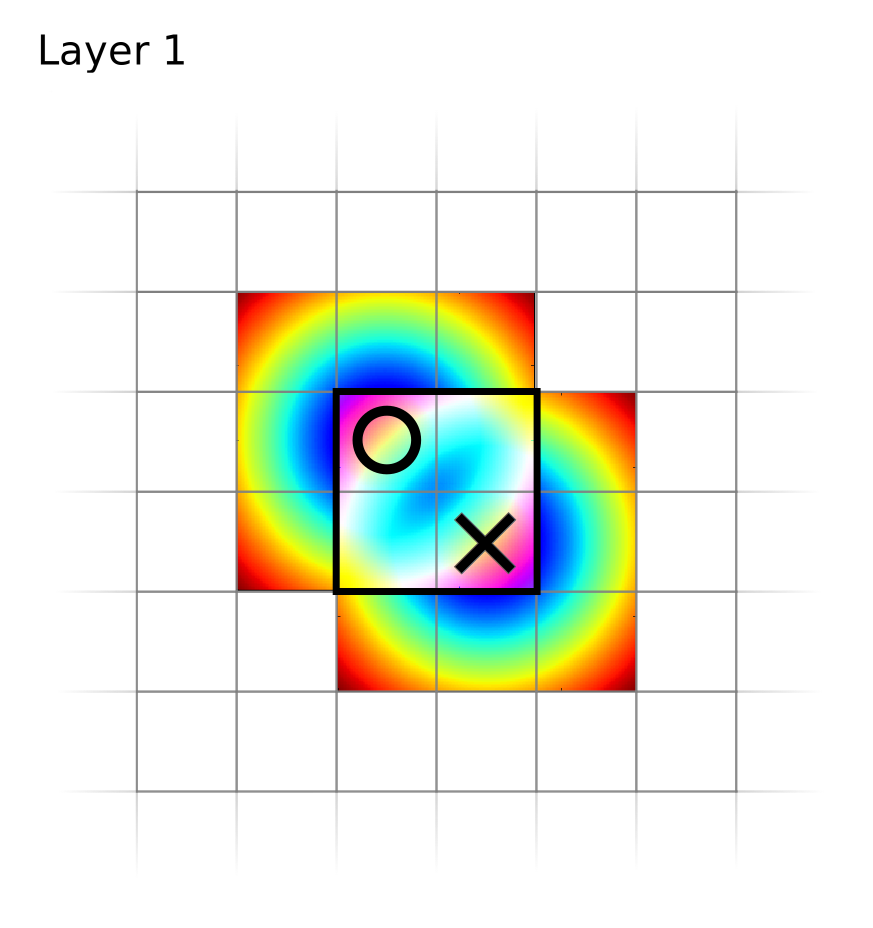
\includegraphics[width=\textwidth]{./coefficient_overlap}
  \caption{Kernel overlap}
  \label{fig:overlap}
  \end{subfigure}
\end{figure}

After this correction algorithm is applied only non-redundant spikes are preserved, this results in a much better reconstruction (Figure \ref{pic-100pc-spikes}). Not only is it more visually pleasing, but the fidelity of the reconstruction has been tested quantitatively; another interesting result is that only 10\% of the rank-ordered and FoCal corrected spikes are needed to preserve 90\% of the visually important information~\cite{basab-thesis}.

\begin{figure}[hbt]
  \centering
  \begin{subfigure}[t]{0.3\textwidth}
    \centering
    \captionsetup{justification=centering,margin=0.1cm}
    \includegraphics[width=\textwidth]{./Lena-gray}
    \caption{Original image}
    \label{pic-original-lena}
  \end{subfigure}
  \begin{subfigure}[t]{0.3\textwidth}
    \centering
    \captionsetup{justification=centering,margin=0.1cm}
    \includegraphics[width=\textwidth]{./final_results-focal-100}
    \caption{100\% of \emph{corrected} spikes}
    \label{pic-100pc-spikes}
  \end{subfigure}
  \begin{subfigure}[t]{0.3\textwidth}
    \centering
    \captionsetup{justification=centering,margin=0.1cm}
    \includegraphics[width=\textwidth]{./final_results-focal-30pc}
    \caption{30\% of \emph{corrected} spikes}
    \label{pic-30pc-spikes}
  \end{subfigure}
  \caption{Results of reconstruction procedure}
  \label{fig-reconstruction}
  \vspace*{-10pt}
\end{figure}



\subsubsection{Implementation details}
Different ways of applying convolutions to images on a GPU where implemented and evaluated. The first one, the \textbf{naïve approach}, implies a discrete convolution with the full 2D kernels. Since we are using squared kernels, this means $N^2 \times W \times H$ operations for a $W\times H$ image using a kernel of width $N$. As expected, performance drops quickly and the biggest problem for this approach was that biggest kernel ($243\times243$ elements) requires more resources than the GPU's constant memory can provide (240 KBytes vs. 64 KBytes). This results in execution errors that may only be fixed using memory with greater latency to store the convolution kernel. 


The second approach to perform a 2D DoG convolution with an image is to rely on \textbf{kernel separability}. A convolution kernel $K$ is said to be \emph{separable} if $K = K_{1} \ast K_{2} \dots K_{n}$. Gaussian kernels are separable (Eq. \ref{eq:Gto1D}). and, fortunately a DoG is merely the subtraction of them (Eq. \ref{eq:DoG2G}).

\begin{equation}
O = I \ast DoG = I \ast G_{c} - I \ast G_{s}
\label{eq:DoG2G}
\end{equation}

Applying the algebraic properties of convolutions and the fact that Gaussian kernels are separable, the full 2D DoG convolution can be performed using four 1D separated ones (Eq. \ref{eq:DoGto1D}).

\begin{equation}
O = I \ast DoG = G_{v,c} \ast G_{h,c} \ast I - G_{v,s} \ast G_{h,s} \ast I 
\label{eq:DoGto1D}
\end{equation}

The main advantage of the separated kernel approach is a reduction of the number of operations needed ($4N\times W \times H$). An exception happens for the $3\times 3$ kernel, in this case there are 12 operations vs. the 9 needed for the naïve approach.


The last approach, \emph{Tiled Convolution} is reported by Advanced Micro Devices (AMD)~\cite{tiled-convolution}. They only present kernels of size $3\times3$, but we have an $11\times11$ convolution working; we are still developing solutions for the larger kernels. 



Convolution alone is a compute intensive task and we obtain about 12 frames-per-second (FPS) on videos with $640\times360$ 8-bit grayscale pixel resolution. Encoding was carried out using a desktop computer running 64-bit GNU/Linux, with a Core i5-4570 4-core CPU @ 3.20~GHz processor with 8~GBytes of 64-bit DDR3 RAM @ 1600~MHz and a GeForce GT 720 GPU with 192 CUDA cores @ 797~MHz, 1~GBytes of 64-bit DDR3 RAM @ 1800~MHz. %\\

\begin{table}[hbt]
  \begin{center}
    \caption{Convolution performance comparison.}
    \bgroup
    \def\arraystretch{1.4}
    \begin{tabular}{l c c c c}
      &
      \begin{minipage}{2cm}\centering Layer 0\vspace*{0.1cm}\end{minipage} & 
      \begin{minipage}{2cm}\centering
        Layer 1\vspace*{0.1cm}\end{minipage}& 
      \begin{minipage}{2cm}\centering
        Layer 2\vspace*{0.1cm}\end{minipage}& 
      \begin{minipage}{2cm}\centering
        Layer 3\vspace*{0.1cm}\end{minipage}\\
      \hline 
      
      Naïve     & 0.0009s & 0.0031s & 0.0587s & N/A$^{1,2}$ \\ 
      Separated & 0.0021s & 0.0055s & 0.0172s & 0.0472s \\ 
      % x, y, 0.01756, 0.04500
      Tiled     & 0.0009s & 0.0044s & 0.1643 & N/A$^2$\\
    \end{tabular} 
    \egroup
    {
      \footnotesize 
      \begin{center}
        $^1$ Unable to fit convolution kernel into constant memory.\\
        $^2$ Unable to compile OpenCL code.
      \end{center}
    }
  \end{center}
  \vspace*{-5pt}
\end{table}

The performance of convolution in GPUs is bound by memory transfers, even if some of the information is reused.



In the retina, redundancy of information is reduced via lateral inhibition 
prior to any ganglion cell activity. In this algorithm, we perform a correction 
on the convolved images by adjusting the pixel values
according to the correlation between convolution kernels 
(Alg.~\ref{code-focal-corr}). The results of using correction 
(Fig.~\ref{pic-unfiltered-spikes}) or not (Fig.~\ref{pic-100pc-spikes}) show 
that the convolution stage can only provide redundant information. Furthermore, 
using only 30\% of the corrected weights still provides enough visual 
information to reconstruct the original image~\cite{basab-model}.

Correcting the spikes for redundancy is a highly time consuming task which
might be better suited for event-based programming, such as the one found on 
the SpiNNaker platform. We are still working on an implementation for this 
approach.\\




12fps is for good most phenomenon, full image encoding

This probably happens only once every so many ms


\subsection{A dynamic vision sensor emulator}

Output what a DVS does but with a camera as a source

Convolution of current and past frames ? centre - current / surround - past

Per-pixel adaptive threshold keeps fast changing pixels from spiking constantly, emulates refractory period of cells.



A second way of encoding is to simulate the early stages of the retina, which 
sense changes in intensity on the photoreceptors. This is quite similar to what 
real Dynamic Vision Sensors (DVS) do but with limited dynamic range and lower 
temporal resolution~\cite{aer-retina-bernabe,dvs-zurich}. The main advantage is 
that no specialized hardware is needed and the operation is so fast that any 
recent computer should be able to do it. For this type of encoding procedure we 
hypothesize that the bigger the change, the sooner a cell would spike and, 
thus, we can obtain a spike timings given the difference of two video frames. 
So far we can process about 20 and 25 FPS using a Numpy and an OpenCL back-end, 
respectively (using the same hardware set-up previously described). Although 
it's currently a good approximation, more research on this algorithm is needed 
to better approximate to biology. 


\section{SpiNNaker implementation}
\input{./chapters/rank_ordered_images/spinnaker_encoding}
\section{Dataset creation}
\input{./chapters/rank_ordered_images/dataset}
%\section{Classification algorithms}
%\input{./chapters/rank_ordered_images/dataset}
\section{Conclusions}
The retina may be seen as a tiny brain that compresses visual input, in that sense it's a very complex organ. Emulating its behaviour is a hard task for general purpose or graphics oriented hardware. The algorithms presented in this section provide a rank-order encoding to video sources. The foveal pit model is able to produce 12 frames per second, and fully encodes the image. The DVS emulator senses spacial and temporal contrast changes in the image and marks them as an event. 

The source code (written in Python and OpenCL) for the foveal-pit model~\cite{focal-code} and the DVS emulator~\cite{pydvs-code} can be found in an online repository.


  \chapter{Conclusions}
  \label{chp:conclusions}
  \section{Conclusion}
\section{Further work}
\section{Plans for second and third year}

  \bibliographystyle{abbrv}
  \bibliography{report-bibliography}

\end{document}
